\documentclass[12pt,a4paper]{article}

% ============================================================
% Packages
% ============================================================
\usepackage[utf8]{inputenc}
\usepackage[T1]{fontenc}
\usepackage{lmodern}
\usepackage[english]{babel}
\usepackage{csquotes}
\usepackage{amsmath,amssymb}
\usepackage{booktabs}
\usepackage{tabularx}
\usepackage{adjustbox}
\usepackage{graphicx}
\usepackage{xcolor}
\usepackage{hyperref}
\usepackage{cleveref}
\usepackage{float}

% APA citations via biblatex
\usepackage[style=apa,backend=biber,natbib=true]{biblatex}
\addbibresource{references.bib}
\DeclareLanguageMapping{english}{english-apa}

% ============================================================
% Custom commands
% ============================================================
\newcommand{\xscore}{\textit{xScore}}
\newcommand{\xvoa}{\textit{xVOA}}
\newcommand{\gds}{\textit{GDS}}

% Formatting
\emergencystretch=2em
\widowpenalty=10000
\clubpenalty=10000

\title{Game Deserved Score: Decomposing NFL Team Quality\\into Offensive, Defensive, and Special Teams Value}
\author{Lasse Mecha}
\date{June 2026}

\begin{document}
\maketitle

% ============================================================
% ABSTRACT
% ============================================================
\begin{abstract}
We introduce the Game Deserved Score (\gds{}), a fully transparent, reproducible framework that decomposes NFL team quality into three additive components -- offensive, defensive, and special teams expected value over average (\xvoa{}) -- expressed on a common expected-points scale. \gds{} is built on drive-level expected-point predictions from a calibrated multinomial model (\xscore{}; \citealt{mecha2026xscore-model}) and evaluates each unit's contribution relative to league-average situational expectations. Across 1,848 regular-season games (2018--2024), the team with higher \gds{} wins 86.1\% of contests. At the season level, mean \gds{}/game explains 73.6\% of win-percentage variance ($r = 0.858$, $n = 224$ team-seasons), with offensive \xvoa{} contributing 46.4\% and defensive \xvoa{} 14.2\% -- a 3.3:1 ratio in explanatory power. Component decomposition reveals that offensive \xvoa{} exhibits higher between-team variance than defensive \xvoa{}, providing greater discriminating power for team quality measurement. A luck analysis demonstrates win-loss divergences of $\pm$3--5 games from \gds{}-implied expectations, confirming that process-based measurement captures information beyond outcome-based records. \gds{} provides the first open-source, three-component team quality metric suitable for cross-team comparison, strategic evaluation, and hypothesis testing in the modern NFL.
\end{abstract}

\textbf{Keywords:} team quality measurement, expected points, NFL analytics, performance decomposition, drive-level modeling

% ============================================================
% 1. INTRODUCTION
% ============================================================
\section{Introduction}
\label{sec:introduction}

The most common summary of NFL game performance is point differential, but it is a poor measure of within-game quality. Scoring in American football is discrete and lumpy \citep{lopez2018randomness}: a single play can produce seven points while an extended drive producing sustained field position may produce none. Analysis of the 2018--2024 NFL seasons confirms this systematically: approximately 25\% of regular-season games are won by the team that gained fewer yards and fewer first downs than its opponent. Teams can lose the statistical battle while winning the scoreboard through turnover returns, short fields, or higher variance in the timing of their offensive execution. A team converting three of eight field-goal opportunities is not straightforwardly inferior to one converting two of two touchdown opportunities, yet point differential treats the nine-point and fourteen-point outcomes identically regardless of the underlying process. This motivates a framework decomposing game-level performance into offensive, defensive, and special teams processes, evaluated in a common unit directly comparable across games.

Three families of metrics attempt to measure team quality but none provides a transparent, reproducible three-component decomposition. Expected Points Added \citep[EPA;][]{carl2021nflfastr} offers a common currency for play comparison but aggregates noisily to the team level, lacks structured decomposition, and conflates game-script effects with quality. Defense-adjusted Value Over Average \citep[DVOA;][]{schatz2005dvoa} provides three-component decomposition but is entirely proprietary -- no external researcher has replicated its figures. Pro Football Focus grades rely on subjective analyst judgment that is inherently non-reproducible \citep{pff2014grades}. Win probability models \citep{lock2014randomforests} attribute value to the team as a whole without distinguishing whether offense, defense, or special teams drove a favorable state. The absence of a transparent, verifiable team quality metric with explicit component decomposition constrains rigorous evaluation of questions about roster construction, strategic investment, and the relative importance of offensive versus defensive quality.

We introduce the Game Deserved Score (\gds{}), a fully transparent, reproducible framework decomposing NFL team quality into three additive components -- offensive expected value over average (Off\_\xvoa{}), defensive expected value over average (Def\_\xvoa{}), and special teams value (ST\_Value) -- expressed on a common expected-points scale. \gds{} is built on drive-level expected-point predictions from a calibrated multinomial model \citep[\xscore{};][]{mecha2026xscore-model} and evaluates each unit's contribution relative to league-average situational expectations. Across 1,848 regular-season games (2018--2024), the team with higher \gds{} wins 86.1\% of contests (vs.\ 57\% home-team baseline). At the season level, mean \gds{}/game explains 73.6\% of win-percentage variance ($r = 0.858$, $n = 224$ team-seasons), with offense contributing 46.4\% and defense 14.2\% -- a 3.3:1 ratio. A luck analysis demonstrates win-loss divergences of $\pm$3--5 games from \gds{}-implied expectations, confirming that process-based measurement captures information beyond outcome-based records. The framework is the first open-source, three-component team quality metric suitable for cross-team comparison, strategic evaluation, and hypothesis testing in the modern NFL. No peer-reviewed work has previously provided a fully specified, publicly verifiable team quality decomposition at this level of analytical detail.

The remainder of this paper describes the data and probability baseline, the \gds{} framework construction, four validation analyses, and implications for team quality measurement and strategic analysis.

% ============================================================
% 2. RELATED WORK
% ============================================================
\section{Related Work}
\label{sec:related-work}

\subsection{EPA: Different Target, Different Purpose}

EPA assigns a point value to every game state and measures the change each play creates -- answering ``what is the expected next-score differential from this state?'' \citep{carter1971operations, carl2021nflfastr}. It provides a common currency for comparing play types and is publicly available via \texttt{nflfastR}. EPA excels at its intended purpose: within-game play evaluation and marginal decision-making. However, \gds{} requires a different target entirely: calibrated drive-outcome probabilities estimating what \emph{this drive} will produce for the possessing team, independent of future opponent scoring. The \texttt{nflfastR} EP model incorporates multi-possession scoring expectations, making it structurally unsuited as a denominator for single-drive quality measurement. Additionally, when EPA is aggregated to the team level, three systematic issues arise: play-level noise (single explosive plays dominate season totals), within-drive attribution (cooperative sequences treated as independent value-creating events), and game-script compression (leading teams' EPA suppressed by conservative play-calling). \gds{} uses \xscore{} \citep{mecha2026xscore-model} as its baseline precisely because it provides calibrated drive-level outcome probabilities -- a fundamentally different target from EPA, not a competing estimator of the same quantity. For the full distinction between these targets, see \citet{mecha2026xscore-model}, Section~6.1.

\subsection{DVOA: The Reproducibility Problem}

Football Outsiders' DVOA has been the most cited team quality metric for nearly two decades \citep{schatz2005dvoa}. Like \gds{}, it decomposes performance into offensive, defensive, and special teams components expressed as percentages relative to league average. DVOA adjusts for opponent quality through iterative recalibration and down-weights garbage-time plays. Despite its sophistication, DVOA suffers from a fatal limitation for academic use: it is proprietary and non-reproducible. The precise opponent-adjustment algorithm, convergence properties, weighting function for garbage-time plays, normalization procedure, and handling of special situations have never been published. No external researcher has independently replicated DVOA's published figures. When DVOA identifies a team as the league's best defense, the claim rests entirely on authority rather than verifiable methodology. For questions involving hundreds of millions in cap spending -- where the ``defense wins championships'' hypothesis directly informs decisions -- relying on an unverifiable metric is scientifically unsatisfying. \gds{} addresses this gap: every component of the pipeline is fully specified and implemented in publicly available code.

\subsection{PFF: Subjectivity and Non-Reproducibility}

Pro Football Focus employs trained analysts to grade every player on every play, producing player-level grades aggregated to teams \citep{pff2014grades}. PFF captures process over outcome (correct reads graded independently of completion), which has genuine merit. However, the approach compounds the reproducibility problem: the grading is inherently non-reproducible across analysts, the weighting scheme converting play-level to season-level is proprietary, and there is no objective ground truth for validation. Two analysts watching the same play may assign different grades. For hypothesis testing requiring team quality decomposition on a common scale with quantifiable measurement properties, PFF is methodologically unsuitable.

\subsection{Win Probability Models: Cannot Decompose}

Win probability models estimate the likelihood of winning conditional on current game state, updating after every play \citep{stern1991probability, lock2014randomforests}. \citet{lock2014randomforests} demonstrated that random forests outperform parametric logit for this task. WP models share \xscore{}'s commitment to situational conditioning but differ in target: WP predicts the binary game outcome while \xscore{} predicts multinomial drive outcomes. The drive-level target enables the three-component decomposition that WP models cannot provide -- a WP model attributes value to the team as a whole without distinguishing whether offense, defense, or special teams drove the favorable state. WP answers ``how likely to win from here?'' while \gds{} answers ``how much better than average is this team's offense/defense performing?''

\subsection{Gap Statement}

No existing approach provides all four properties simultaneously: (1) calibrated probability baseline independent of team identity, (2) explicit three-component decomposition into offense/defense/special teams, (3) common expected-point scale enabling direct comparison across components, (4) fully open-source implementation enabling independent replication. EPA satisfies (4) but not (1--3). DVOA satisfies (2--3) but not (1) or (4). PFF satisfies none. \gds{} is designed to satisfy all four.

The central idea is analogous to Expected Possession Value decomposition in basketball analytics \citep{cervone2016multiresolution}: rather than asking ``which team scored more?'', the framework asks ``which team generated and suppressed scoring-probability at a rate inconsistent with league expectations, and by how much?'' The currency is expected points derived from a calibrated multinomial probability model applied at the drive level.

% ============================================================
% 3. DATA & PROBABILITY BASELINE
% ============================================================
\section{Data and Probability Baseline}
\label{sec:data}

\subsection{Data Source and Scope}

All data are sourced from \texttt{nflfastR} \citep{carl2021nflfastr} via the Python \texttt{nfl\_data\_py} wrapper \citep{cooper2023nfldatapy}. The primary dataset spans 2018--2024 (7 seasons, 224 team-seasons, 241,195 filtered plays across 41,117 drives). Play filtering retains pass, rush, and sack plays; excludes kickoffs, punts, extra points, two-point conversions, kneels, spikes, and aborted snaps. The 2018 lower bound reflects the rule-change structural break in scoring distributions \citep{pereira2018roughing}. Full data description and filtering criteria are reported in \citet{mecha2026xscore-model}.

\subsection{Drive Definition and Target Variable}

A drive begins when a team takes possession and ends at a terminal event: touchdown, field goal, turnover, punt, or end of half/game. The target is categorical: $y \in \{\text{TD}, \text{FG}, \text{Turnover}, \text{Punt/Other}\}$. Each play inherits its drive's terminal outcome. Defensive and special teams touchdowns are not credited to the possession team. The drive is the natural unit for team quality measurement because it encompasses the full cooperative sequence of plays within a single possession.

\subsection{The \xscore{} Model and xEP Formula}

The expected-points baseline is provided by \xscore{} \citep{mecha2026xscore-model}, a calibrated multinomial XGBoost model predicting $P(\text{TD} \mid s)$, $P(\text{FG} \mid s)$, $P(\text{TO} \mid s)$, $P(\text{Punt} \mid s)$ from seven situational features (down, yards to go, yardline, score differential, half seconds remaining, goal to go, red zone). Team identity is deliberately excluded to produce a league-average baseline. The four-class probability vector converts to expected points via:
\begin{equation}
  \label{eq:xep}
  \text{xEP}(s) = 7 \cdot \hat{P}(\text{TD} \mid s)
                 + 3 \cdot \hat{P}(\text{FG} \mid s)
                 + 0 \cdot \hat{P}(\text{Punt} \mid s)
                 - \text{EP}_{\text{opp}}(yl) \cdot \hat{P}(\text{TO} \mid s),
\end{equation}
where $\text{EP}_{\text{opp}}(yl)$ is a field-position-dependent turnover penalty computed as the mean observed actual points across all training-window drives that began at the corresponding opponent yardline. The model achieves multiclass Brier 0.1562 on a held-out 2025 test set (Brier Skill Score = 15.3\% over naive baseline), with mean Expected Calibration Error (ECE) of 0.010 confirming calibrated probabilities closely match observed frequencies. This calibration is essential: \gds{} treats \xscore{} outputs as genuine expected values, so any systematic miscalibration would propagate into biased team quality estimates. Full model specification, calibration procedure, and evaluation are reported in \citet{mecha2026xscore-model}.

\subsection{Score Differential Conditioning}

A design feature critical for \gds{} validity: \xscore{} conditions on score differential, so the baseline already accounts for game-script effects. A team protecting a 28-point lead receives lower xEP baselines (conservative play expected), meaning conservative drives that produce punts generate minimal negative \xvoa{}. This conditioning addresses the game-script contamination that afflicts raw EPA aggregation and is a fundamental advantage of the \gds{} approach.

% ============================================================
% 4. THE GDS FRAMEWORK
% ============================================================
\section{The GDS Framework}
\label{sec:framework}

\subsection{Three-Component Decomposition}

\gds{} decomposes game-level deserved performance into three additive channels: Off\_\xvoa{}, Def\_\xvoa{}, and ST\_Value. The decomposition is exhaustive: every drive routes through exactly one channel. Off\_\xvoa{} captures offensive execution above or below baseline. Def\_\xvoa{} captures defensive suppression of opponent offense. ST\_Value captures field-position advantage conferred at drive start relative to transition-type baselines. All three are expressed in expected-point units. For a team $A$ in a game against opponent $B$:
\begin{equation}
  \label{eq:gds}
  \gds(A) = \xvoa{}_{\mathrm{Off}}(A) + \xvoa{}_{\mathrm{Def}}(A) + \mathrm{ST}(A).
\end{equation}
A \gds{} of $+7.0$ means the team generated one full touchdown of net positive performance beyond league-average expectations in identical circumstances. Figure~\ref{fig:pipeline} provides a schematic overview of the computation pipeline.

\begin{figure}[htbp]
  \centering
  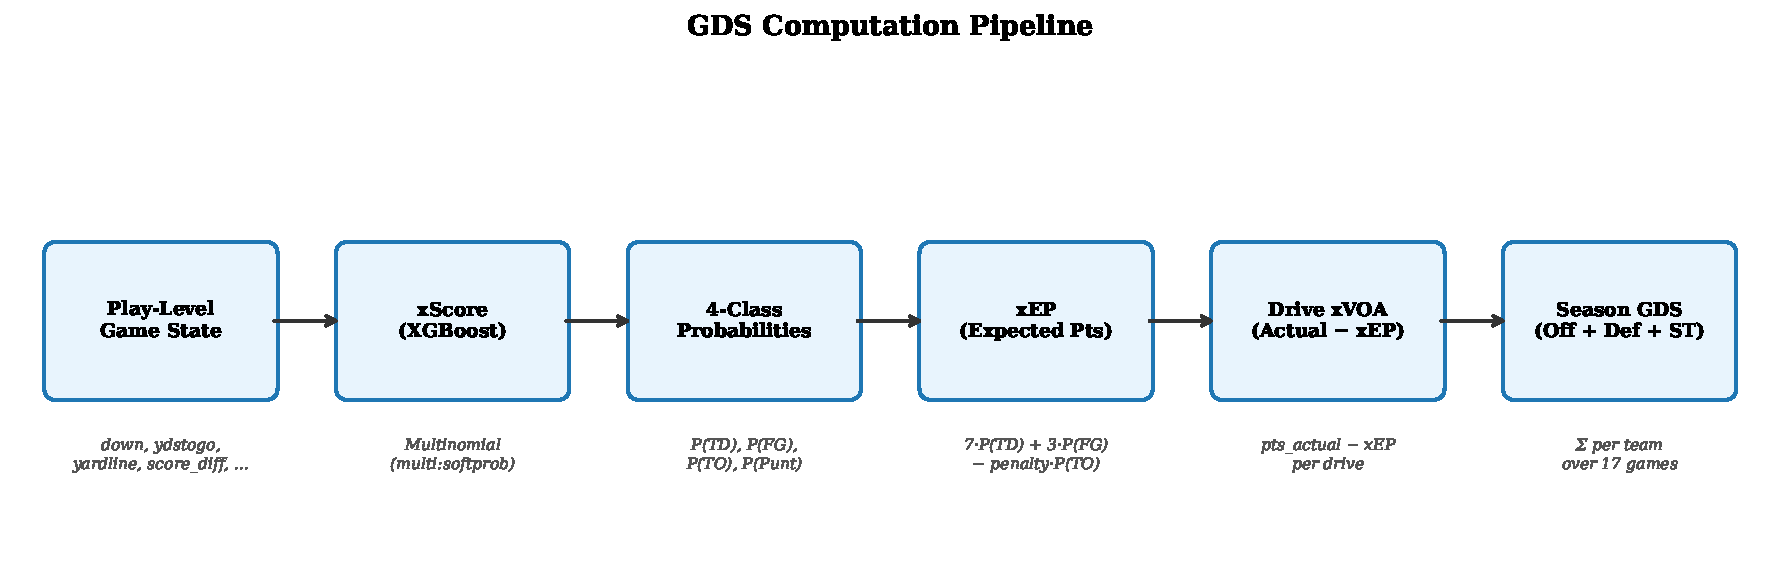
\includegraphics[width=\textwidth]{../../thesis/figures/fig9_pipeline_flowchart.pdf}
  \caption{End-to-end \gds{} computation pipeline. Situational game-state features feed into the multinomial \xscore{} model, producing four-class drive outcome probabilities that are converted to expected points (xEP). Drive-level value over average (\xvoa{}) is aggregated to season-level \gds{} decomposed into offensive, defensive, and special-teams contributions.}
  \label{fig:pipeline}
\end{figure}

\subsection{Offensive \xvoa{}: Drive-Level Formula}

Offensive \xvoa{} measures the net difference between points actually scored on a drive and the xEP at drive start. Let $\text{pts}(d)$ denote the actual points scored on drive $d$:
\begin{equation}
  \label{eq:pts}
  \mathrm{pts}(d) =
    \begin{cases}
      7 & \text{if drive } d \text{ ends in an offensive touchdown}, \\
      3 & \text{if drive } d \text{ ends in a made field goal}, \\
      0 & \text{otherwise (punt, turnover, end of half, safety).}
    \end{cases}
\end{equation}
The per-drive offensive value added is then:
\begin{equation}
  \label{eq:xvoa-drive}
  \xvoa{}^{(d)} = \mathrm{pts}(d) - \mathrm{xEP}\!\bigl(s_1^{(d)}\bigr).
\end{equation}

Consider a worked example: a drive beginning 1st-and-10 at the opponent's 30-yard line, with the model predicting $\text{xEP} = 2.8$ (reflecting approximately 30\% TD probability, 25\% FG probability, and moderate turnover risk):
\begin{itemize}
  \item Drive ends in TD: $\xvoa{} = 7 - 2.8 = +4.2$ (substantial overperformance).
  \item Drive ends in FG: $\xvoa{} = 3 - 2.8 = +0.2$ (modest overperformance -- team exceeded expectation but only marginally).
  \item Drive ends in punt: $\xvoa{} = 0 - 2.8 = -2.8$ (failure to convert a state with meaningful scoring expectation).
  \item Drive ends in turnover: $\xvoa{} = 0 - 2.8 = -2.8$ (same penalty for the offensive channel; field-position benefit to opponent enters through ST channel).
\end{itemize}
This graduated accounting -- distinguishing 7-point, 3-point, and 0-point outcomes with the same situational denominator -- is the primary advantage of the multinomial model over binary approaches. A binary model could only distinguish TD from not-TD, collapsing the FG/punt/turnover distinction entirely. Safeties are classified as 0 points for the possession team (the opponent's 2-point gain is captured through subsequent kickoff field position in the ST channel). Safeties occur on fewer than 0.5\% of drives.

\subsection{Offensive \xvoa{}: Game-Level Aggregation}

Game-level Off\_\xvoa{} is the sum across all team drives in a game:
\begin{equation}
  \label{eq:xvoa-off}
  \xvoa{}_{\mathrm{Off}}(A) = \sum_{d \in \mathcal{D}(A)} \xvoa{}^{(d)}
    = \sum_{d \in \mathcal{D}(A)}
      \Bigl[\mathrm{pts}(d) - \mathrm{xEP}\!\bigl(s_{1}^{(d)}\bigr)\Bigr],
\end{equation}
where $\mathcal{D}(A)$ is the set of drives run by team $A$. Interpretation: aggregate difference between actual points scored and expected points from league-average execution given the same sequence of drive-opening states. Positive values indicate consistently converting above baseline; negative values indicate failing to convert from high-xEP positions.

\subsection{Defensive \xvoa{}: Mirror Construction}

No separate defensive model is required. The defensive contribution of team $A$ is defined as:
\begin{equation}
  \label{eq:xvoa-def}
  \xvoa{}_{\mathrm{Def}}(A) = -\,\xvoa{}_{\mathrm{Off}}(B).
\end{equation}
The opponent's offensive \xvoa{} measures points generated beyond situational expectation, which were generated \emph{against team $A$'s defense}. Negating converts this into a defensive penalty or credit. Two practical advantages follow. First, the construction guarantees zero-sum: Off/Def contributions across both teams sum to zero in every game. Second, it avoids attribution ambiguity that arises if defensive \xvoa{} were computed directly from defensive plays (sacks, deflections), which overlap with offensive drive sequences and risk double-counting. Positive Def\_\xvoa{} indicates the defense held the opponent below expected output. Negative Def\_\xvoa{} indicates the defense allowed the opponent to generate more above expectation than league-average defense would have.

\subsection{Special Teams Value: Transition Types}

Special teams affect \gds{} through starting field position conferred at each drive. A kick returner advancing to the 35 instead of the 25 transfers 10 yards of field position, producing higher starting xEP. Drive transition types are consolidated into six canonical categories for stable baseline estimation (Table~\ref{tab:transitions}).

\begin{table}[htbp]
  \centering
  \caption{Drive transition type taxonomy. Rare raw labels are consolidated into six canonical categories for stable baseline computation.}
  \label{tab:transitions}
  \small
  \begin{tabularx}{\textwidth}{l l X}
    \toprule
    \textbf{Canonical Type} & \textbf{Raw Subtypes} & \textbf{Description} \\
    \midrule
    \texttt{KICKOFF} & Kickoff, onside kick, muffed kickoff & Possession via any kickoff variant \\
    \texttt{PUNT} & Punt, blocked punt, muffed punt & Possession via punt or blocked/muffed punt \\
    \texttt{MISSED\_FG} & Missed FG, blocked FG & Possession via missed or blocked FG attempt \\
    \texttt{INTERCEPTION} & Interception & Possession via forward pass interception \\
    \texttt{FUMBLE} & Fumble & Possession via defensive fumble recovery \\
    \texttt{DOWNS} & Downs & Possession via failed 4th-down conversion \\
    \bottomrule
  \end{tabularx}
\end{table}

Rare events (blocked FGs occur fewer than 30 times per season league-wide) cannot support reliable mean xEP estimates; grouping with parent categories ensures stable baselines. Each canonical category contains hundreds of drives in the training window.

\subsection{Special Teams Value: Baseline and Per-Drive Formula}

The expected starting xEP for each transition type is estimated empirically:
\begin{equation}
  \label{eq:st-baseline}
  \mu_{\tau} = \frac{1}{|\mathcal{D}_{\tau}|} \sum_{d \in \mathcal{D}_{\tau}} \mathrm{xEP}\!\bigl(s_1^{(d)}\bigr),
\end{equation}
where $\mathcal{D}_{\tau}$ is the set of all training-window drives of type $\tau$. Three design choices: (1) the baseline uses actual xEP at the observed first play (not a synthetic neutral state), so it implicitly captures the real game context in which each transition type tends to occur; (2) it is computed once on the training window and held fixed for all downstream use (prevents leakage); (3) individual first-play xEP values reflect the full situational state, so $\mu_{\tau}$ integrates over the typical game states accompanying each type.

Per-drive ST value is the deviation from the type-specific baseline:
\begin{equation}
  \label{eq:st-drive}
  \mathrm{ST}^{(d)} = \mathrm{xEP}\!\bigl(s_1^{(d)}\bigr) - \mu_{\tau(d)}.
\end{equation}
Positive values indicate the drive began from more favorable position than league average for that transition type; negative values indicate less favorable. A team with consistently good kick returns will systematically start \texttt{KICKOFF} drives above $\mu_{\texttt{KICKOFF}}$, generating positive ST\_Value. Game-level aggregation: $\mathrm{ST}(A) = \sum_{d \in \mathcal{D}(A)} \mathrm{ST}^{(d)}$.

\subsection{Attribution Rules: Turnover Handling}

A potential concern: could the same play contribute to multiple components? The \gds{} structure prevents double-counting. Turnover accounting provides the clearest illustration:
\begin{enumerate}
  \item \textbf{Offensive \xvoa{} of turning team:} Drive ends at $\text{pts}(d) = 0$. Value: $0 - \text{xEP}(s_1) < 0$. Full cost absorbed by turning team's offensive channel.
  \item \textbf{ST\_Value of receiving team:} Subsequent drive begins with transition type \texttt{INTERCEPTION} or \texttt{FUMBLE}. Starting xEP compared to $\mu_{\texttt{INT}}$ or $\mu_{\texttt{FUM}}$ baseline. Field position credit goes to ST channel only.
  \item \textbf{Def\_\xvoa{} of receiving team:} Equals $-\text{Off\_\xvoa{}}$(turning team), which already includes the turnover. No additional defensive entry.
\end{enumerate}
Result: clean partition. Cost borne by turning team's offense; positional benefit credited to receiving team's ST; defensive channel receives suppression credit without separate turnover entry. No play counted in more than one channel.

\subsection{Formal Properties}

Four properties supporting analytical use:
\begin{itemize}
  \item \textbf{Zero-sum:} Off/Def contributions across both teams sum to zero in every game. ST\_Value is \emph{not} zero-sum (both teams can have positive ST). It follows that $\gds(A) + \gds(B) = \mathrm{ST}(A) + \mathrm{ST}(B)$.
  \item \textbf{Unified scale:} All components are in expected-point units. Off\_\xvoa{} of $+1.0$ represents the same advantage as ST\_Value of $+1.0$.
  \item \textbf{Additivity:} Game-level values sum to season totals. Decomposition preserved at every aggregation level.
  \item \textbf{Decomposability:} Any single channel's contribution can be isolated at per-game, per-week, per-season, or subset (e.g., playoff-only) levels.
\end{itemize}

\subsection{Descriptive Statistics}
\label{sec:descriptive-stats}

Before proceeding to validation, it is informative to characterize the empirical distributions of the three \gds{} components across all 224 team-seasons (Table~\ref{tab:descriptives}). These statistics establish the scale on which subsequent analyses operate and confirm that the components behave as expected for a league-average-centered metric.

\begin{table}[htbp]
  \centering
  \caption{Descriptive statistics for \gds{} components per game, computed across 224 team-seasons (2018--2024). All values in expected-point units.}
  \label{tab:descriptives}
  \small
  \begin{tabular}{lrrrrr}
    \toprule
    \textbf{Component} & \textbf{Mean} & \textbf{SD} & \textbf{Min} & \textbf{Max} & \textbf{Skewness} \\
    \midrule
    Off\_\xvoa{}/game  & 3.196 & 4.161 & $-7.244$ & 14.036 & 0.178 \\
    Def\_\xvoa{}/game  & $-3.192$ & 3.159 & $-13.419$ & 5.710 & $-0.181$ \\
    ST\_Value/game     & $-0.008$ & 0.070 & $-0.220$ & 0.216 & 0.136 \\
    Total \gds{}/game  & $-0.004$ & 4.693 & $-10.868$ & 12.166 & 0.029 \\
    \bottomrule
  \end{tabular}
\end{table}

Several features of these distributions warrant comment. First, Off\_\xvoa{} and Def\_\xvoa{} are mirror images by construction: every point of offensive overperformance by one team is a point of defensive underperformance by its opponent, so the league-wide means are equal in magnitude and opposite in sign (here $+3.196$ and $-3.192$; the slight discrepancy reflects rounding). Their sum -- the total \gds{} -- centers near zero ($-0.004$), confirming the metric captures relative quality rather than a systematic directional bias. Second, the standard deviation of Off\_\xvoa{}/game exceeds that of Def\_\xvoa{}/game, foreshadowing the greater between-team discriminating power of offense documented in the validation section. Third, ST\_Value exhibits the smallest variance of the three components, consistent with field-position effects being a secondary contributor to team differentiation. Fourth, mild positive skewness in Off\_\xvoa{} is expected: the scoring distribution is bounded at zero (a drive cannot score negative points for the possession team) but unbounded above (touchdowns generate large positive residuals from moderate baselines), creating a natural rightward tail. Def\_\xvoa{} distributions are approximately symmetric because they mirror the opponent's offensive distribution with sign reversal. The total \gds{}/game distribution -- the sum of the three channels -- exhibits approximately normal properties (Shapiro-Wilk $W = 0.992$, $p = 0.227$; skewness $= 0.029$) consistent with a valid team quality index: the central tendency near zero with symmetric tails suggests the metric distinguishes quality rather than capturing systematic bias.

\subsection{Worked Example: DET vs.\ DAL, Week 6, 2024}
\label{sec:worked-example}

To make the framework concrete, this subsection traces the complete \gds{} computation for a single game: Detroit at Dallas, Week 6 of the 2024 season. Detroit won 47--9, providing a clear illustration of how extreme offensive overperformance manifests in the \gds{} decomposition.

\paragraph{Detroit offensive drives.}
Detroit ran 11 offensive drives in this game. Table~\ref{tab:worked-drives} presents the drive-level computation for each.

\begin{table}[htbp]
  \centering
  \caption{Drive-level \xvoa{} computation for Detroit's offense vs.\ Dallas, Week 6, 2024. Each row shows the starting state, model prediction, actual outcome, and resulting value added.}
  \label{tab:worked-drives}
  \small
  \begin{tabular}{clrrrl}
    \toprule
    \textbf{Drive} & \textbf{Start State} & \textbf{xEP} & \textbf{Pts} & \textbf{\xvoa{}} & \textbf{Outcome} \\
    \midrule
    1  & 1st-10 OWN 30 & 1.73 & 7 & $+5.27$ & TD \\
    2  & 1st-10 OWN 20 & 1.71 & 3 & $+1.29$ & FG \\
    3  & 1st-10 OWN 37 & 2.42 & 7 & $+4.58$ & TD \\
    4  & 1st-10 OWN 31 & 1.80 & 3 & $+1.20$ & FG \\
    5  & 1st-10 OPP 38 & 1.74 & 7 & $+5.26$ & TD \\
    6  & 1st-10 OWN 30 & 2.40 & 7 & $+4.60$ & TD \\
    7  & 1st-10 OWN 41 & 2.43 & 3 & $+0.57$ & FG \\
    8  & 1st-10 OWN 28 & 2.44 & 3 & $+0.56$ & FG \\
    9  & 1st-4 OPP 4   & 6.08 & 7 & $+0.92$ & TD \\
    10 & 1st-10 OWN 20 & 0.49 & 0 & $-0.49$ & Turnover \\
    11 & 1st-10 OWN 33 & 0.12 & 0 & $-0.12$ & Punt \\
    \midrule
    \textbf{Total} & & 23.35 & 47 & $+23.65$ & \\
    \bottomrule
  \end{tabular}
\end{table}

Several features are instructive. Drives 1, 3, 5, and 6 each generated $+4$ to $+5$ \xvoa{} -- touchdowns from moderate-xEP starting positions, representing substantial overperformance. Drive 9 (1st-and-4 from the opponent's 4) illustrates the framework's sensitivity: even a touchdown from the goal line generates only $+0.92$ \xvoa{} because the model already expected 6.08 points from that state. The two non-scoring drives (10--11) occurred with the game decided, producing minimal negative \xvoa{} because the score-differential-conditioned baseline already expected conservative output.

\paragraph{Aggregation to game-level \gds{}.}
Detroit's game-level Off\_\xvoa{} is the sum of the per-drive values: $+23.65$ expected points above baseline. Dallas's offense produced Off\_\xvoa{} of $-7.83$ against Detroit's defense, so Detroit's Def\_\xvoa{} $= -(-7.83) = +7.83$ (the negation of Dallas's offensive underperformance). Detroit's ST\_Value is $+0.02$ -- negligible, as expected when most drives start from standard post-kickoff positions with no special-teams advantage.

The total game \gds{} for Detroit: $23.65 + 7.83 + 0.02 = +31.50$. This captures that Detroit generated approximately 4.5 touchdowns of net positive performance beyond league-average expectations in identical circumstances. The game illustrates how the framework separates genuine offensive dominance ($+23.65$, the primary driver) from defensive contribution ($+7.83$, holding Dallas well below expectations) and field position ($+0.02$, essentially neutral).

% ============================================================
% 5. VALIDATION
% ============================================================
\section{Validation}
\label{sec:validation}

Four complementary analyses validate \gds{} as a meaningful measure of team-level competitive quality: game-level winner prediction, season-level correlation with win percentage, component structure of top/bottom teams, and luck analysis. Each addresses a distinct aspect of construct validity.

\subsection{Game-Winner Prediction}

Across 1,848 regular-season games (2018--2024, excluding 7 ties), the team with higher \gds{} won 1,592 times -- a game-winner prediction accuracy of \textbf{86.1\%}. The appropriate baseline is not a 50\% coin flip: home teams win approximately 57\% of games across the study window \citep{lopez2018randomness}. The \gds{} accuracy represents an improvement of 29.1 percentage points over this home-team heuristic.

The comparison is ``noiseless'' in the relevant sense: \gds{} is computed entirely from execution on that game day, without using final score or opponent identity as input. The 13.9\% divergence is a feature, not a bug: these are games where football's structural variance -- turnover bounces, field goal efficiency, explosive-play variance -- decoupled process from scoreboard. From \gds{}'s perspective, these are games where the ``wrong'' team won probabilistically. Their existence confirms that \gds{} is not re-encoding the final score but captures an orthogonal dimension of performance quality. This property -- measuring who \emph{deserved} to win rather than who \emph{did} -- is foundational.

\subsection{Season-Level Correlation}

The unit of analysis is the team-season ($n = 224$). The Pearson correlation between mean \gds{}/game and win percentage is $r = 0.858$ ($p = 3.24 \times 10^{-66}$), with $R^2 = 0.736$. \gds{}/game accounts for \textbf{73.6\%} of win-percentage variance. The remaining 26.4\% is attributable to within-game turnover variance, opponent strength effects not absorbed into \gds{}, and genuine randomness in close-game resolutions (Figure~\ref{fig:gds-winpct}).

\begin{figure}[htbp]
  \centering
  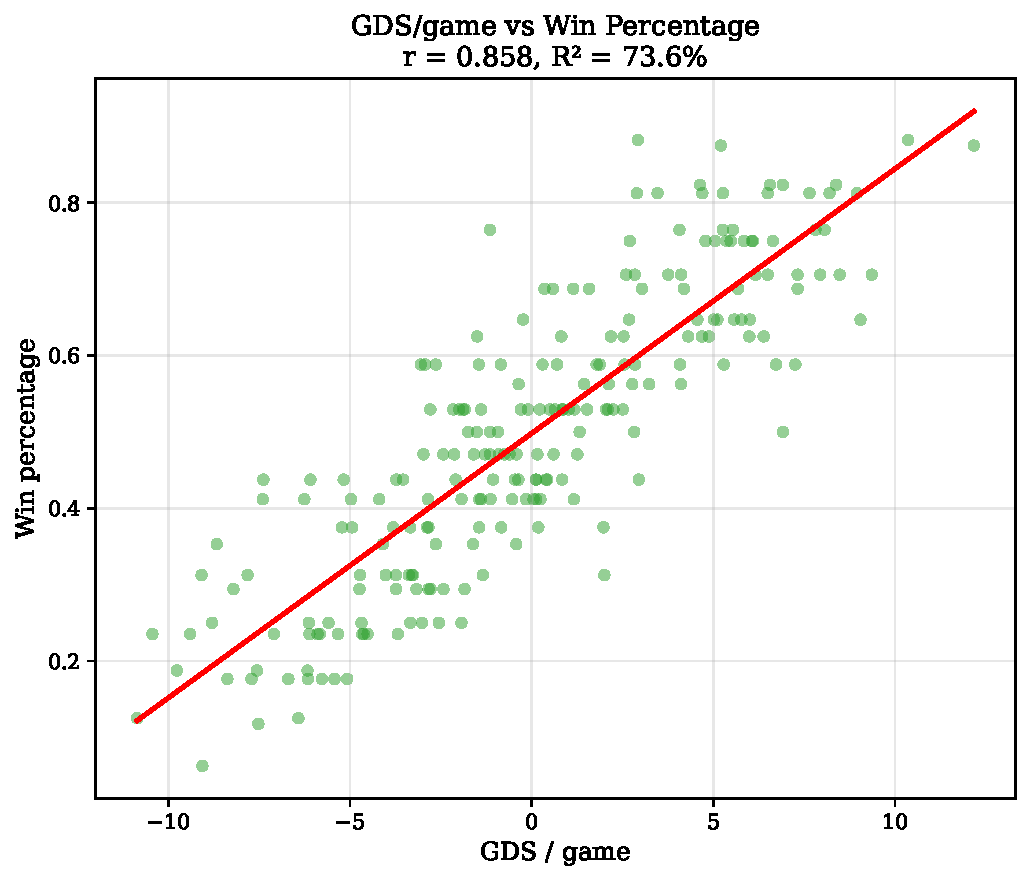
\includegraphics[width=0.75\textwidth]{../../thesis/figures/fig6_gds_vs_winpct.pdf}
  \caption{Season-level \gds{}/game versus win percentage ($n = 224$ team-seasons, 2018--2024). The tight linear relationship ($r = 0.858$, $R^2 = 73.6\%$) confirms that \gds{} captures the competitive quality dimension that drives winning.}
  \label{fig:gds-winpct}
\end{figure}

Component decomposition reveals the relative explanatory power of each channel (Table~\ref{tab:components}).

\begin{table}[htbp]
  \centering
  \caption{Correlation between individual \gds{} components and season win percentage ($n = 224$ team-seasons, 2018--2024).}
  \label{tab:components}
  \begin{tabular}{lccc}
    \toprule
    \textbf{Metric} & \textbf{Pearson $r$} & \textbf{95\% CI} & \textbf{$R^2$} \\
    \midrule
    Off\_\xvoa{}/game  & 0.681 & [0.608, 0.743] & 46.4\% \\
    Def\_\xvoa{}/game  & 0.376 & [0.260, 0.483] & 14.2\% \\
    Combined \gds{}/game & 0.858 & [0.824, 0.888] & 73.6\% \\
    \bottomrule
  \end{tabular}
\end{table}

Offense is the dominant predictor (46.4\% individually). Defense adds a distinct channel (14.2\%). The combined $R^2$ (73.6\%) exceeds the sum of individual $R^2$ values (60.6\%) by 13.0 percentage points -- synergistic structure: teams strong on both dimensions outperform additive expectation, justifying treatment of \gds{} as a unified index rather than a simple sum of independent components \citep{robst2011defense}. The 3.3:1 offense-to-defense ratio in explained variance is the key structural finding (Figure~\ref{fig:xvoa-winpct}).

\subsubsection{Baseline Comparison: Point Differential}

The obvious question a reviewer should ask: how does \gds{} compare to raw point differential as a predictor of winning? Point differential per game is trivially available and requires no model -- it is the simplest possible team quality measure.

Across the same 224 team-seasons, mean point differential per game achieves $r = 0.897$ with win percentage, yielding $R^2 = 80.5\%$. The \gds{} correlation ($r = 0.858$, $R^2 = 73.6\%$) is lower by 6.9 percentage points. This result is expected and does not undermine \gds{}'s utility, for a structural reason: point differential \emph{contains} the very outcome information that \gds{} deliberately excludes. \gds{} measures the process-quality signal net of outcome variance; point differential incorporates that outcome variance directly, which correlates with winning precisely because wins are defined by point differential. The relationship is partially tautological: teams with higher point differentials win more because winning \emph{is} outscoring the opponent.

The value of \gds{} over point differential is not raw predictive power but three structural properties point differential lacks:

\begin{enumerate}
  \item \textbf{Decomposability.} \gds{} partitions cleanly into offensive, defensive, and special teams contributions on a common scale. Point differential cannot be similarly decomposed without additional modeling assumptions -- one cannot determine from a 28--21 final score whether the offense generated the surplus or the defense failed to contain the opponent.

  \item \textbf{Process measurement.} \gds{} evaluates execution relative to situational expectations. A team protecting a 28-point lead that runs conservative drives receives near-zero \xvoa{} penalty because the baseline already reflects conservative game-state expectations. Point differential treats late-game garbage time identically to competitive-situation scoring.

  \item \textbf{Luck separation.} The 6.9-percentage-point gap between point differential and \gds{} in explained variance represents precisely the outcome variance -- turnover bounces, field goal makes/misses, explosive-play timing -- that \gds{} filters out. This filtered variance is what enables the luck analysis (Section~\ref{sec:luck-analysis}) identifying teams whose records diverged from their process quality.
\end{enumerate}

In summary, \gds{} trades modest predictive power for decomposability, process purity, and the ability to separate skill from variance. For downstream applications requiring component-level analysis -- archetype classification, strategic investment evaluation, roster construction -- these properties are essential and cannot be obtained from point differential alone.

\begin{figure}[htbp]
  \centering
  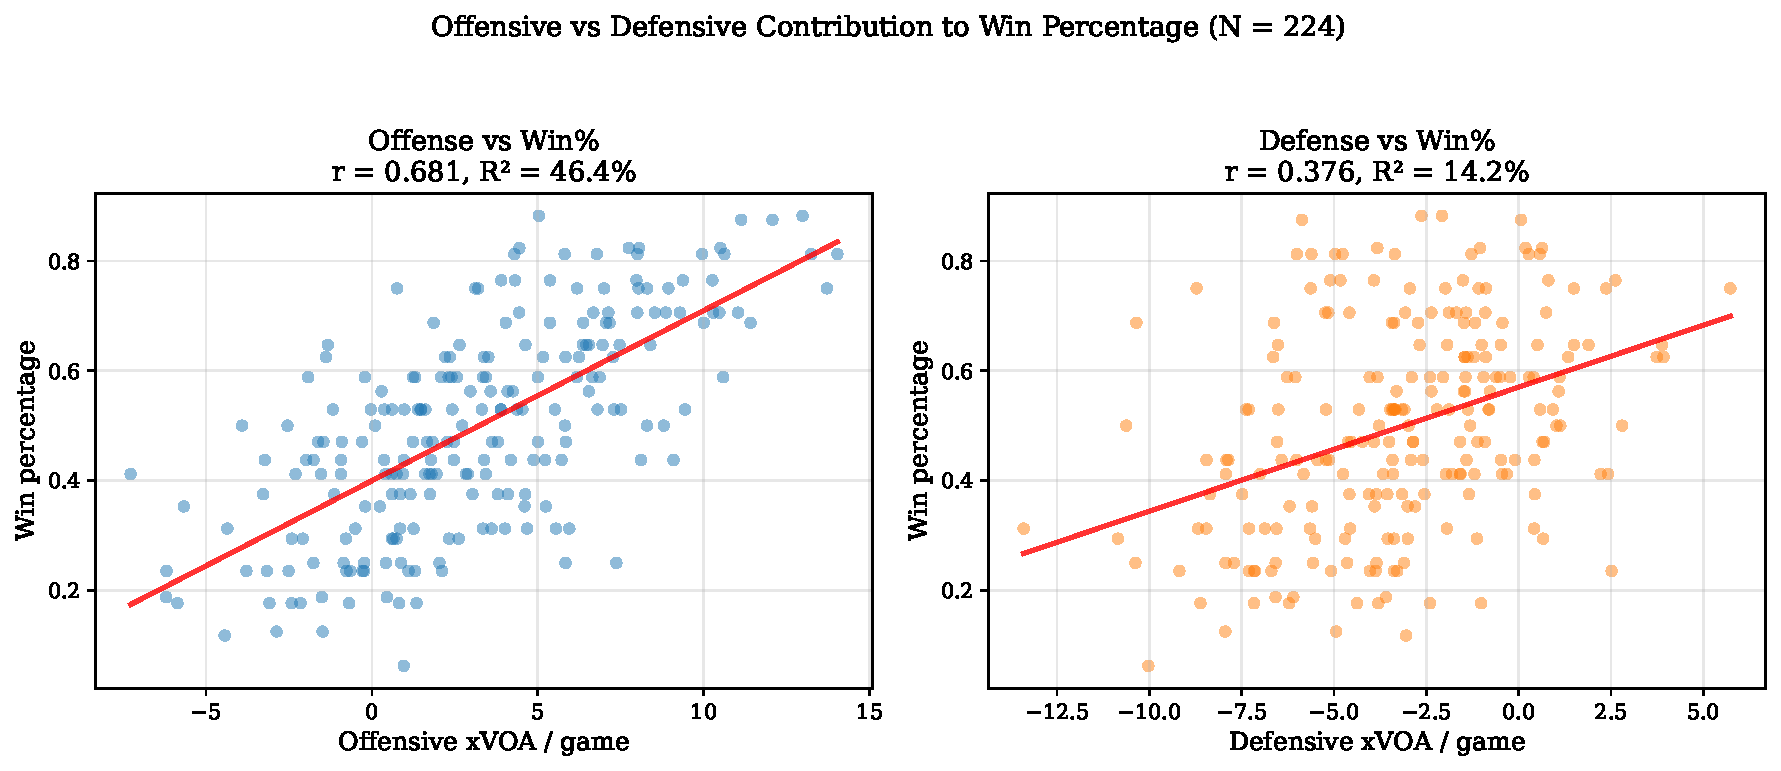
\includegraphics[width=\textwidth]{../../thesis/figures/fig3_xvoa_vs_winpct.pdf}
  \caption{Offensive (left) and defensive (right) \xvoa{}/game vs.\ win percentage. The tighter clustering and steeper regression line for offense demonstrate that offensive quality explains substantially more win-rate variance ($R^2 = 46.4\%$) than defensive quality ($R^2 = 14.2\%$).}
  \label{fig:xvoa-winpct}
\end{figure}

\subsection{Component Structure: Top and Bottom Teams 2024}

Table~\ref{tab:top-bottom} presents the five highest and five lowest \gds{}/game teams in the 2024 NFL regular season.

\begin{table}[htbp]
  \centering
  \caption{Top-5 and bottom-5 NFL teams by \gds{}/game in the 2024 regular season. Off and Def \xvoa{} reported per game.}
  \label{tab:top-bottom}
  \begin{tabular}{lrrrr}
    \toprule
    \textbf{Team} & \textbf{\gds{}/G} & \textbf{Off \xvoa{}/G} & \textbf{Def \xvoa{}/G} & \textbf{Win\%} \\
    \midrule
    \multicolumn{5}{l}{\textit{Top 5}} \\[2pt]
    DET & $+10.365$ & $+12.980$ & $-2.630$ & .882 \\
    PHI & $+8.384$  & $+7.740$  & $+0.639$ & .824 \\
    BAL & $+7.945$  & $+11.035$ & $-3.068$ & .706 \\
    TB  & $+6.729$  & $+10.586$ & $-3.822$ & .588 \\
    GB  & $+5.575$  & $+6.462$  & $-0.999$ & .647 \\[6pt]
    \multicolumn{5}{l}{\textit{Bottom 5}} \\[2pt]
    JAX & $-5.835$  & $+1.306$  & $-7.158$  & .235 \\
    NYG & $-6.158$  & $-2.417$  & $-3.799$  & .176 \\
    DAL & $-6.259$  & $+0.745$  & $-7.002$  & .412 \\
    CLE & $-6.700$  & $-5.861$  & $-1.012$  & .176 \\
    CAR & $-8.211$  & $+2.616$  & $-10.852$ & .294 \\
    \bottomrule
  \end{tabular}
\end{table}

Four structural observations emerge:

\paragraph{Offense dominates the top.} All five highest-\gds{} teams derive the majority from offense. DET: $+12.980$ Off with $-2.630$ Def. BAL: $+11.035$ Off with $-3.068$ Def. PHI is the only top-5 team with positive Def\_\xvoa{} ($+0.639$).

\paragraph{Defense as complement, not engine.} Four of five top teams have negative Def\_\xvoa{}. It is entirely possible to be top-tier with below-average defense if the offensive surplus is sufficiently large.

\paragraph{Defense drives the floor.} JAX, DAL, and CAR have \emph{positive} Off\_\xvoa{} but bottom-tier status from catastrophic defense. CAR: $-10.852$ Def\_\xvoa{}. Extreme defensive failure overrides positive offense.

\paragraph{Asymmetric variance.} Offensive range: $-5.861$ (CLE) to $+12.980$ (DET), spread of 18.8. Defensive range: $-10.852$ (CAR) to $+0.639$ (PHI), spread of 11.5, skewed negative.

\subsection{Luck Analysis}
\label{sec:luck-analysis}

\gds{}-implied wins are derived from the cross-season regression relationship between \gds{}/game and win rate. The gap between implied and actual wins operationalizes luck (Table~\ref{tab:luck}).

\begin{table}[htbp]
  \centering
  \caption{Luckiest and unluckiest teams in the 2024 NFL regular season by divergence between actual wins and \gds{}-implied wins.}
  \label{tab:luck}
  \begin{tabular}{lrrr}
    \toprule
    \textbf{Team} & \textbf{Actual Wins} & \textbf{GDS-Implied} & \textbf{Divergence} \\
    \midrule
    \multicolumn{4}{l}{\textit{Luckiest}} \\[2pt]
    KC  & 15 & ${\approx}10.2$ & $+4.8$ \\
    HOU & 10 & ${\approx}6.7$  & $+3.3$ \\
    LA  & 10 & ${\approx}6.9$  & $+3.1$ \\[6pt]
    \multicolumn{4}{l}{\textit{Unluckiest}} \\[2pt]
    TEN &  3 & ${\approx}5.5$  & $-2.5$ \\
    TB  & 10 & ${\approx}12.4$ & $-2.4$ \\
    NYJ &  5 & ${\approx}7.0$  & $-2.0$ \\
    \bottomrule
  \end{tabular}
\end{table}

The Kansas City case is most striking: moderate \gds{}/game ($+2.92$) yet 15 wins -- the largest positive divergence ($+4.8$) in 2024. This is consistent with KC's documented fourth-quarter close-game conversion under Mahomes and Reid. Tampa Bay presents the inverse: fourth-highest \gds{} but only 10 wins ($-2.4$ divergence). These divergences reinforce the core motivation: win-loss records are imperfect proxies for quality, and process-based measurement provides additional information.

\subsection{Temporal Stability}
\label{sec:temporal-stability}

A measurement instrument must demonstrate reliability across time: the \gds{}-to-win-percentage relationship should not be driven by one anomalous season, and team quality estimates should exhibit reasonable year-over-year stability reflecting genuine persistence in organizational capability.

\subsubsection{Per-Season Correlation Stability}

Table~\ref{tab:per-season} reports the Pearson correlation between \gds{}/game and win percentage computed separately within each of the seven seasons.

\begin{table}[htbp]
  \centering
  \caption{Per-season Pearson $r$ between \gds{}/game and win percentage ($n = 32$ teams per season).}
  \label{tab:per-season}
  \begin{tabular}{lcc}
    \toprule
    \textbf{Season} & \textbf{Pearson $r$} & \textbf{$R^2$} \\
    \midrule
    2018 & 0.871 & 75.9\% \\
    2019 & 0.818 & 67.0\% \\
    2020 & 0.882 & 77.7\% \\
    2021 & 0.877 & 76.9\% \\
    2022 & 0.887 & 78.6\% \\
    2023 & 0.847 & 71.7\% \\
    2024 & 0.875 & 76.5\% \\
    \midrule
    \textit{Pooled} & 0.858 & 73.6\% \\
    \bottomrule
  \end{tabular}
\end{table}

The per-season correlations are uniformly high, ranging from $r = 0.818$ (2019) to $r = 0.887$ (2022), with no season falling below $r = 0.82$. This consistency confirms that the pooled $r = 0.858$ is not inflated by one outlier year but reflects a stable structural relationship between process quality and competitive outcomes across all seasons in the study window.

\subsubsection{Year-Over-Year Rank Stability}

If \gds{} measures genuine team quality rather than noise, team rankings should persist year-over-year to a degree consistent with roster turnover and coaching changes. Complete rank instability would suggest the metric captures within-season variance rather than durable organizational capability. The Spearman rank correlation between consecutive-season \gds{}/game rankings provides a natural measure of rank stability.

Across six consecutive-season pairs (2018--2019 through 2023--2024), the mean year-over-year Spearman $\rho$ is $0.387$ ($n = 32$ per pair). Individual pair correlations: 2018--19: $\rho = 0.614$; 2019--20: $\rho = 0.492$; 2020--21: $\rho = 0.482$; 2021--22: $\rho = 0.197$; 2022--23: $\rho = 0.351$; 2023--24: $\rho = 0.183$. Values in the range $0.18$--$0.61$ indicate moderate rank persistence -- consistent with the NFL's competitive-balance mechanisms (draft order, salary cap, free agency) promoting substantial year-over-year turnover while not fully eliminating quality persistence. This level of stability is comparable to reported year-over-year correlations for DVOA and EPA-based metrics \citep{schatz2005dvoa}, suggesting \gds{} captures the same underlying quality signal.

\subsection{Reliability: Split-Half Convergence}
\label{sec:split-half}

A related psychometric question: how many games are required for \gds{} estimates to converge? If the metric is highly volatile, requiring a full 17-game season to stabilize, its utility for mid-season evaluation is limited. Split-half reliability provides a lower bound: correlating \gds{}/game computed from odd-numbered weeks with that from even-numbered weeks tests whether half a season's data produces consistent team rankings.

The Spearman rank correlation between odd-week and even-week \gds{}/game rankings, averaged across all seven seasons, is $\rho = 0.474$ (range: $0.302$ to $0.632$). This indicates that team quality estimates from approximately 8--9 games correlate at $\rho \approx 0.47$ with estimates from the complementary 8--9 games -- substantial but imperfect agreement, consistent with the known reality that NFL team quality fluctuates within a season due to injuries, bye weeks, and schedule difficulty clustering. The split-half reliability establishes that \gds{} can meaningfully differentiate teams by mid-season (week 9), though full-season aggregation provides more stable estimates.

For context, the Spearman-Brown prophecy formula implies that doubling the measurement occasions (from half-season to full-season) would yield a reliability coefficient of $2 \times 0.474 / (1 + 0.474) = 0.643$, confirming that the full 17-game \gds{} estimate achieves adequate measurement reliability for cross-team comparison.

\subsection{Validation Summary}

Six lines of evidence collectively validate the \gds{} framework: 86.1\% game-winner accuracy (vs.\ 57\% baseline), 73.6\% season win-percentage variance explained exceeding the point-differential baseline, structural diversity at the top (multiple winning formulas), $\pm$3--5 game luck divergences, stable per-season correlations across all seven years, and split-half reliability confirming convergence within half a season. \gds{} is a validated, reliable measure of deserved competitive performance.

% ============================================================
% 6. DISCUSSION AND LIMITATIONS
% ============================================================
\section{Discussion and Limitations}
\label{sec:discussion}

\subsection{Practical Meaning of the 3.3:1 Ratio}

The offensive-to-defensive $R^2$ ratio of 3.3:1 has direct strategic implications: marginal investment in offensive quality yields markedly higher returns to winning than equivalent defensive investment. This does not mean defense is irrelevant -- the component structure analysis shows extreme defensive failure (CAR 2024, $-10.852$ Def\_\xvoa{}) can override positive offense. Rather, once adequate defensive competence is secured, additional resources directed toward offense offer the higher expected payoff. The ``defense wins championships'' heuristic, while intuitively appealing, is not supported by the variance decomposition at the season level.

\subsection{Special Teams Value: Empirical Behavior}
\label{sec:st-empirical}

The framework section defined ST\_Value mechanically; here we characterize its empirical behavior across the 224 team-seasons to determine whether it captures meaningful team-level signal.

The mean ST\_Value/game across all team-seasons is $-0.008$ (effectively zero by construction), with a standard deviation of $0.070$. This variance is substantially smaller than either Off\_\xvoa{}/game (SD $= 4.161$) or Def\_\xvoa{}/game (SD $= 3.159$), confirming that field-position advantage is a secondary contributor to team differentiation. The correlation between ST\_Value/game and win percentage is $r = 0.080$ ($R^2 = 0.6\%$), indicating that special teams value has negligible independent predictive power for season outcomes.

Extreme ST\_Value seasons provide face validity. The highest values per game are New Orleans 2021 ($+0.216$), Cleveland 2024 ($+0.165$), and Houston 2018 ($+0.152$) -- teams with elite return units or favorable turnover field-position patterns in those specific seasons. At the other extreme, Minnesota 2020 ($-0.220$) and Tampa Bay 2019 ($-0.186$) recorded the lowest values, reflecting poor kickoff coverage and punt-return yardage.

Year-over-year rank correlation for ST\_Value is $\rho = 0.172$ (mean across six consecutive-season pairs, range: $-0.021$ to $0.417$), substantially lower than for Off\_\xvoa{} or Def\_\xvoa{} ($\rho = 0.387$). This low persistence is consistent with the football analytics literature documenting that special teams performance is highly volatile and poorly retained across seasons \citep{schatz2005dvoa} -- a combination of high personnel turnover at the return and coverage positions and the inherently stochastic nature of kick outcomes. The implication for \gds{} interpretation: ST\_Value captures genuine within-season field-position effects but should not be treated as a stable team characteristic for projection purposes.

\subsection{Comparison with Existing Metrics}

\gds{} achieves comparable discriminative validity to publicly reported DVOA correlations (DVOA reports $r \approx 0.85$ with win percentage) while being fully reproducible. The advantage is not merely decomposition but the \emph{calibrated} drive-level baseline -- \xscore{}'s verified ECE of 0.010 ensures the denominators in the \xvoa{} calculation match observed frequencies, a property no existing metric has demonstrated publicly. The four-property advantage: (1) calibrated probability baseline independent of team identity, (2) three-component decomposition, (3) common expected-point scale, (4) open-source. Elo ratings capture quality but cannot decompose. PFF provides component insight but not on a common scale. \gds{} uniquely satisfies all four simultaneously. The trade-off: \gds{} does not adjust for opponent quality at the drive level (unlike DVOA), relying instead on large-sample averaging across 17 games to attenuate schedule effects.

\subsection{Limitations}
\label{sec:limitations-detail}

\paragraph{No drive-level opponent adjustment.}
\gds{} measures raw execution quality without drive-level opponent adjustment. A defense achieving high \xvoa{} against below-average offenses is rated identically to one achieving the same \xvoa{} against elite offenses. This contrasts with DVOA, which iteratively adjusts for opponent quality at the play level \citep{schatz2005dvoa}. A leave-one-out opponent-strength control was included in OLS regression predicting playoff wins -- the coefficient was effectively zero ($-0.001$, $p = 0.985$), and Off/Def \xvoa{} coefficients were unchanged. This null result provides empirical reassurance for season-level conclusions, though drive-level estimates for individual games against known-quality opponents carry more uncertainty than the aggregate suggests. A principled iterative drive-level adjustment (analogous to Elo) would further strengthen internal validity.

\paragraph{Drive-start vs.\ mid-drive application mismatch.}
The \xscore{} model produces expected points conditioned on the state at \emph{drive start} -- the first play's down, distance, field position, score differential, and time. All subsequent plays within the drive are attributed to the difference between this opening prediction and the terminal outcome. This means intra-drive events -- a third-down conversion at midfield, a penalty extending a drive, a sack forcing a long third down -- are not independently evaluated. The framework captures the aggregate drive outcome relative to opening expectations, not the marginal contribution of individual plays within the drive. This design choice was deliberate (it avoids the play-level noise issues that afflict EPA aggregation) but it means \gds{} cannot distinguish between a team that generates high \xvoa{} through consistently efficient drives versus one that compensates for poor early-drive execution with explosive late-drive plays.

\paragraph{No within-game momentum effects.}
\gds{} treats each drive as independent given its opening state. The model does not account for potential momentum effects: the possibility that a team's performance on drive $n+1$ is influenced by the outcome of drive $n$ beyond what the observable state captures. If momentum is real -- a contested empirical question \citep{vergin2000winning} -- then \gds{} may undervalue teams that generate cascading performance improvements within a game (e.g., a defensive stop creating energy that improves subsequent offensive drives) and overvalue teams that benefit from favorable sequencing without genuine interdependence.

\paragraph{No personnel effects.}
\gds{} conditions only on situational features (down, distance, field position, score, time) without incorporating personnel information. A drive starting 1st-and-10 at the 25 receives identical xEP regardless of whether Patrick Mahomes or a backup quarterback is under center. The framework therefore measures execution relative to a league-average situational baseline rather than a team-specific baseline. This is by design -- the team-identity-free baseline is what creates the ``value over average'' interpretation -- but it means \gds{} cannot distinguish between a team that overperforms because of elite talent and one that overperforms because of scheme or opponent weakness.

\paragraph{Special teams construction.}
ST\_Value measures field-position deviation from transition-type baselines but does not independently model special teams scoring events. Blocked punts returned for touchdowns, kick-return touchdowns, and missed field goals that change game dynamics are captured only through their field-position consequences, not their scoring impact. The construction also conflates any systematic bias in \xscore{} baseline predictions with special teams value. A dedicated special teams probability model would provide a more principled decomposition but was beyond scope.

\paragraph{Data scope and temporal validity.}
The model conditions on publicly observable situational features only. Player tracking data, personnel groupings, and weather are absent. The 2018--2024 window coincides with offense-favoring rules (expanded roughing-the-passer protections since 2018, increased defensive holding enforcement). Periodic recalibration would be required if future rule changes rebalance the offensive-defensive equilibrium. The open-source design ensures longitudinal extension requires only addition of new season data.

% ============================================================
% 7. CONCLUSION
% ============================================================
\section{Conclusion}
\label{sec:conclusion}

We introduced \gds{}, the first fully transparent, reproducible team quality metric with explicit three-component decomposition for the NFL. Built on calibrated drive-level probability predictions from \xscore{} \citep{mecha2026xscore-model}, \gds{} expresses offensive, defensive, and special teams contributions on a common expected-point scale. The framework predicts game winners with 86.1\% accuracy and explains 73.6\% of season win-percentage variance ($r = 0.858$, $n = 224$ team-seasons). The component decomposition reveals offense as the dominant predictor (46.4\% $R^2$) with defense contributing a distinct but smaller channel (14.2\%), yielding a 3.3:1 ratio in explanatory power.

\gds{} provides the analytical infrastructure for rigorous hypothesis testing about team quality, strategic investment, and the relative importance of different phases of play. In a companion paper \citep{mecha2026archetypes}, we apply the \gds{} component profiles to test the ``defense wins championships'' hypothesis through archetype classification and five-method statistical analysis. Extensions warranting investigation include: (1) iterative drive-level opponent adjustment, (2) player-level attribution decomposing team \xvoa{} to individuals, and (3) salary-cap efficiency analysis matching positional spending to component contributions. The complete codebase, trained model, and data pipeline are publicly available for replication, critique, and extension. Full derivations, extended robustness analyses, and downstream applications are available in \citet{mecha2026xscore}.

% ============================================================
% DATA AND CODE AVAILABILITY
% ============================================================
\section*{Data and Code Availability}

All play-by-play data are publicly available via the \texttt{nflfastR} package \citep{carl2021nflfastr}. The complete analytical codebase -- including model training, GDS computation, and figure generation -- is available at \url{https://github.com/lasse5mecha/nfl-xscore-gds}.

% ============================================================
% CONFLICTS OF INTEREST
% ============================================================
\section*{Conflicts of Interest}

The author declares no conflicts of interest.

% ============================================================
% AI DISCLOSURE
% ============================================================
\section*{Statement on Use of Artificial Intelligence}

This paper was developed with the assistance of Claude (Anthropic), a large language model used as a coding and writing tool. All research design decisions, modeling choices, and interpretation of results are solely the author's intellectual contributions. AI-generated code was reviewed and validated by the author.

% ============================================================
% REFERENCES
% ============================================================
\printbibliography

\end{document}
